% Options for packages loaded elsewhere
\PassOptionsToPackage{unicode,citecolor=black}{hyperref}
\PassOptionsToPackage{hyphens}{url}
\PassOptionsToPackage{dvipsnames,svgnames,x11names}{xcolor}
%
\documentclass[
  authoryear,
  preprint,
  1p]{elsarticle}

\usepackage{amsmath,amssymb}
\usepackage{iftex}
\ifPDFTeX
  \usepackage[T1]{fontenc}
  \usepackage[utf8]{inputenc}
  \usepackage{textcomp} % provide euro and other symbols
\else % if luatex or xetex
  \usepackage{unicode-math}
  \defaultfontfeatures{Scale=MatchLowercase}
  \defaultfontfeatures[\rmfamily]{Ligatures=TeX,Scale=1}
\fi
\usepackage{lmodern}
\ifPDFTeX\else  
    % xetex/luatex font selection
\fi
% Use upquote if available, for straight quotes in verbatim environments
\IfFileExists{upquote.sty}{\usepackage{upquote}}{}
\IfFileExists{microtype.sty}{% use microtype if available
  \usepackage[]{microtype}
  \UseMicrotypeSet[protrusion]{basicmath} % disable protrusion for tt fonts
}{}
\makeatletter
\@ifundefined{KOMAClassName}{% if non-KOMA class
  \IfFileExists{parskip.sty}{%
    \usepackage{parskip}
  }{% else
    \setlength{\parindent}{0pt}
    \setlength{\parskip}{6pt plus 2pt minus 1pt}}
}{% if KOMA class
  \KOMAoptions{parskip=half}}
\makeatother
\usepackage{xcolor}
\setlength{\emergencystretch}{3em} % prevent overfull lines
\setcounter{secnumdepth}{5}
% Make \paragraph and \subparagraph free-standing
\makeatletter
\ifx\paragraph\undefined\else
  \let\oldparagraph\paragraph
  \renewcommand{\paragraph}{
    \@ifstar
      \xxxParagraphStar
      \xxxParagraphNoStar
  }
  \newcommand{\xxxParagraphStar}[1]{\oldparagraph*{#1}\mbox{}}
  \newcommand{\xxxParagraphNoStar}[1]{\oldparagraph{#1}\mbox{}}
\fi
\ifx\subparagraph\undefined\else
  \let\oldsubparagraph\subparagraph
  \renewcommand{\subparagraph}{
    \@ifstar
      \xxxSubParagraphStar
      \xxxSubParagraphNoStar
  }
  \newcommand{\xxxSubParagraphStar}[1]{\oldsubparagraph*{#1}\mbox{}}
  \newcommand{\xxxSubParagraphNoStar}[1]{\oldsubparagraph{#1}\mbox{}}
\fi
\makeatother


\providecommand{\tightlist}{%
  \setlength{\itemsep}{0pt}\setlength{\parskip}{0pt}}\usepackage{longtable,booktabs,array}
\usepackage{calc} % for calculating minipage widths
% Correct order of tables after \paragraph or \subparagraph
\usepackage{etoolbox}
\makeatletter
\patchcmd\longtable{\par}{\if@noskipsec\mbox{}\fi\par}{}{}
\makeatother
% Allow footnotes in longtable head/foot
\IfFileExists{footnotehyper.sty}{\usepackage{footnotehyper}}{\usepackage{footnote}}
\makesavenoteenv{longtable}
\usepackage{graphicx}
\makeatletter
\def\maxwidth{\ifdim\Gin@nat@width>\linewidth\linewidth\else\Gin@nat@width\fi}
\def\maxheight{\ifdim\Gin@nat@height>\textheight\textheight\else\Gin@nat@height\fi}
\makeatother
% Scale images if necessary, so that they will not overflow the page
% margins by default, and it is still possible to overwrite the defaults
% using explicit options in \includegraphics[width, height, ...]{}
\setkeys{Gin}{width=\maxwidth,height=\maxheight,keepaspectratio}
% Set default figure placement to htbp
\makeatletter
\def\fps@figure{htbp}
\makeatother

\makeatletter
\@ifpackageloaded{caption}{}{\usepackage{caption}}
\AtBeginDocument{%
\ifdefined\contentsname
  \renewcommand*\contentsname{Table of contents}
\else
  \newcommand\contentsname{Table of contents}
\fi
\ifdefined\listfigurename
  \renewcommand*\listfigurename{List of Figures}
\else
  \newcommand\listfigurename{List of Figures}
\fi
\ifdefined\listtablename
  \renewcommand*\listtablename{List of Tables}
\else
  \newcommand\listtablename{List of Tables}
\fi
\ifdefined\figurename
  \renewcommand*\figurename{Figure}
\else
  \newcommand\figurename{Figure}
\fi
\ifdefined\tablename
  \renewcommand*\tablename{Table}
\else
  \newcommand\tablename{Table}
\fi
}
\@ifpackageloaded{float}{}{\usepackage{float}}
\floatstyle{ruled}
\@ifundefined{c@chapter}{\newfloat{codelisting}{h}{lop}}{\newfloat{codelisting}{h}{lop}[chapter]}
\floatname{codelisting}{Listing}
\newcommand*\listoflistings{\listof{codelisting}{List of Listings}}
\makeatother
\makeatletter
\makeatother
\makeatletter
\@ifpackageloaded{caption}{}{\usepackage{caption}}
\@ifpackageloaded{subcaption}{}{\usepackage{subcaption}}
\makeatother
\journal{JASA-EL}

\ifLuaTeX
  \usepackage{selnolig}  % disable illegal ligatures
\fi
\usepackage[]{natbib}
\bibliographystyle{elsarticle-harv}
\usepackage{bookmark}

\IfFileExists{xurl.sty}{\usepackage{xurl}}{} % add URL line breaks if available
\urlstyle{same} % disable monospaced font for URLs
\hypersetup{
  pdftitle={A conceptual framework for the practical use of predictive models and Soundscape Indices: Goals, constraints, and applications},
  pdfauthor={Andrew Mitchell; Francesco Aletta; Tin Oberman; Mercede Erfanian; Jian Kang},
  pdfkeywords={Soundscape, Predictive Modelling, Auditory
Environment, ISO12913},
  colorlinks=true,
  linkcolor={blue},
  filecolor={Maroon},
  citecolor={Blue},
  urlcolor={Blue},
  pdfcreator={LaTeX via pandoc}}


\setlength{\parindent}{6pt}
\begin{document}

\begin{frontmatter}
\title{A conceptual framework for the practical use of predictive models
and Soundscape Indices: Goals, constraints, and applications}
\author[1]{Andrew Mitchell%
\corref{cor1}%
}
 \ead{andrew.mitchell.18@ucl.ac.uk} 
\author[1]{Francesco Aletta%
%
}
 \ead{f.aletta@ucl.ac.uk} 
\author[1]{Tin Oberman%
%
}
 \ead{t.oberman@ucl.ac.uk} 
\author[1]{Mercede Erfanian%
%
}
 \ead{mercede.erfanianghasab.18@ucl.ac.uk} 
\author[1]{Jian Kang%
%
}
 \ead{j.kang@ucl.ac.uk} 

\affiliation[1]{organization={University College London, Institute for
Environmental Design and Engineering},addressline={Central House, 14
Upper Woburn Place},city={London},postcode={WC1H 0NN},postcodesep={}}

\cortext[cor1]{Corresponding author}





        
\begin{abstract}
With the recent standardization of soundscape, there has been increased
interest in bringing the soundscape approach into an engineering
context. While traditional assessment methods, such as those given in
the ISO 12913 series, provide information on the current status quo of
an environment, they offer limited insight into hypothetical
environments and are therefore less relevant for design purposes. This
conference paper presents a conceptual framework for the practical use
of predictive soundscape models and indices. The framework outlines the
goals, constraints, and potential applications of these models and
highlights the need for further research in this area to better
understand the dynamics of soundscape perception and to put predictive
models to practical use. Predictive soundscape models can be integrated
with soundscape indices - such as those being developed by the
Soundscape Indices (SSID) project - for assessment purposes, providing a
comprehensive approach to evaluating and designing sound environments.
The use of predictive models is necessary to address the challenges
faced in practical applications of the soundscape approach and to fill
the gap between traditional assessment methods and the design of sound
environments.
\end{abstract}





\begin{keyword}
    Soundscape \sep Predictive Modelling \sep Auditory Environment \sep 
    ISO12913
\end{keyword}
\end{frontmatter}
    

\section{Introduction}\label{introduction}

As the future of urban sound research and practice moves toward a more
holistic soundscape focus, the ability to affect change at large scales
and in a wide range of projects will require that familiar engineering
tools and approaches can be applied to soundscape design. When
attempting to apply soundscape in practice in the built environment, it
becomes apparent that a predictive model of the users' perceptual
response to the acoustic environment is necessary. Whether to determine
the impact of a design change, or to integrate a large scale data at
neighbourhood and city levels, a mathematical model of the interacting
factors will form a vital component of the implementation of the
soundscape approach.

Current methods of assessing soundscapes are generally limited to a post
hoc assessment of the existing environment, where users of the space in
question are surveyed regarding their experience of the acoustic
environment \citep{Engel2018Review, Zhang2018Effect, Ba2019Effect}.
While this approach has proved useful in identifying the impacts of an
existing environment, designers require the ability to predict how a
change or proposed design will impact the soundscape of the space,
before its implementation. To this end, a model that is built on
measurable or estimate-able quantities of the environment would
represent a leap forward in the ability to design soundscapes and to
assess their broad impacts on health and wellbeing.

We will begin by outlining the use cases of predictive soundscape models
and how they are necessary for certain applications. From the desired
use cases, we will then outline a framework within which practical
predictive models can be developed.

\section{Defining what a predictive soundscape model
is}\label{defining-what-a-predictive-soundscape-model-is}

\citet{Aletta2016Soundscape} provide a review of the soundscape
descriptors and indicators commonly used in soundscape research and
outlines an initial framework for developing predictive soundscape
models. In their review, the authors identified eight potential
soundscape descriptors, including perceived affective quality
\citep{Axelsson2010principal}, restorativeness
\citep{Payne2013production}, etc. Similarly, the authors identified a
range of potential indicators used to characterise the acoustic
environment, including environmental acoustics indicators such as
\(L_{Aeq}\), \(L_{Ceq} − L_{Aeq}\) and psychoacoustic indicators such as
Loudness (\(N_5\)) and Sharpness (S).

However, it is noted that several studies show that no single
psychoacoustic indicator alone can explain the variation in soundscape
responses (as expressed via the descriptors) (e.g.
\citep{PerssonWaye2002Psycho}). The goal of statistical modelling,
therefore is to create a more complex and complete representation of the
relationship between soundscape indicators and descriptors, beyond what
any single indicator could achieve.

Figure~\ref{fig-model} shows a conceptual view of this relationship. We
start with \textbf{soundscape indicators}, which characterise the
physical and contextual environment to which the listener is exposed.
This can be broken down into \textbf{sonic features} (e.g.~the
acoustical features listed above) and \textbf{characteristics of the
space itself} (e.g.~the amount of visible sky, the intended use-case of
the space, how crowded the space is, etc.). In order to translate from
the physical inputs to an expressed description of the soundscape
perception, we introduce the concept of a \textbf{perceptual mapping}
\citep{Lionello2021new}. This mapping represents a simplified idea of
how each individual's brain processes the inputs from the soundscape
which they experience, forms a perception, and finally expresses that
perception through their description of the soundscape. For our
purposes, this perceptual mapping is treated as essentially a black box
mapping inputs to outputs. It can be conceived of as a network of
weights in which certain characteristics of the sound may have different
weights and directions depending on the context, through which all of
the inputs are processed, resulting in the soundscape rating.
Conceptually, this perceptual mapping -- the pathways and weightings
through which the inputs are processed before being expressed as a
perceptual descriptor -- is established prior to an individual's
exposure to the soundscape in question.

\begin{figure}

\centering{

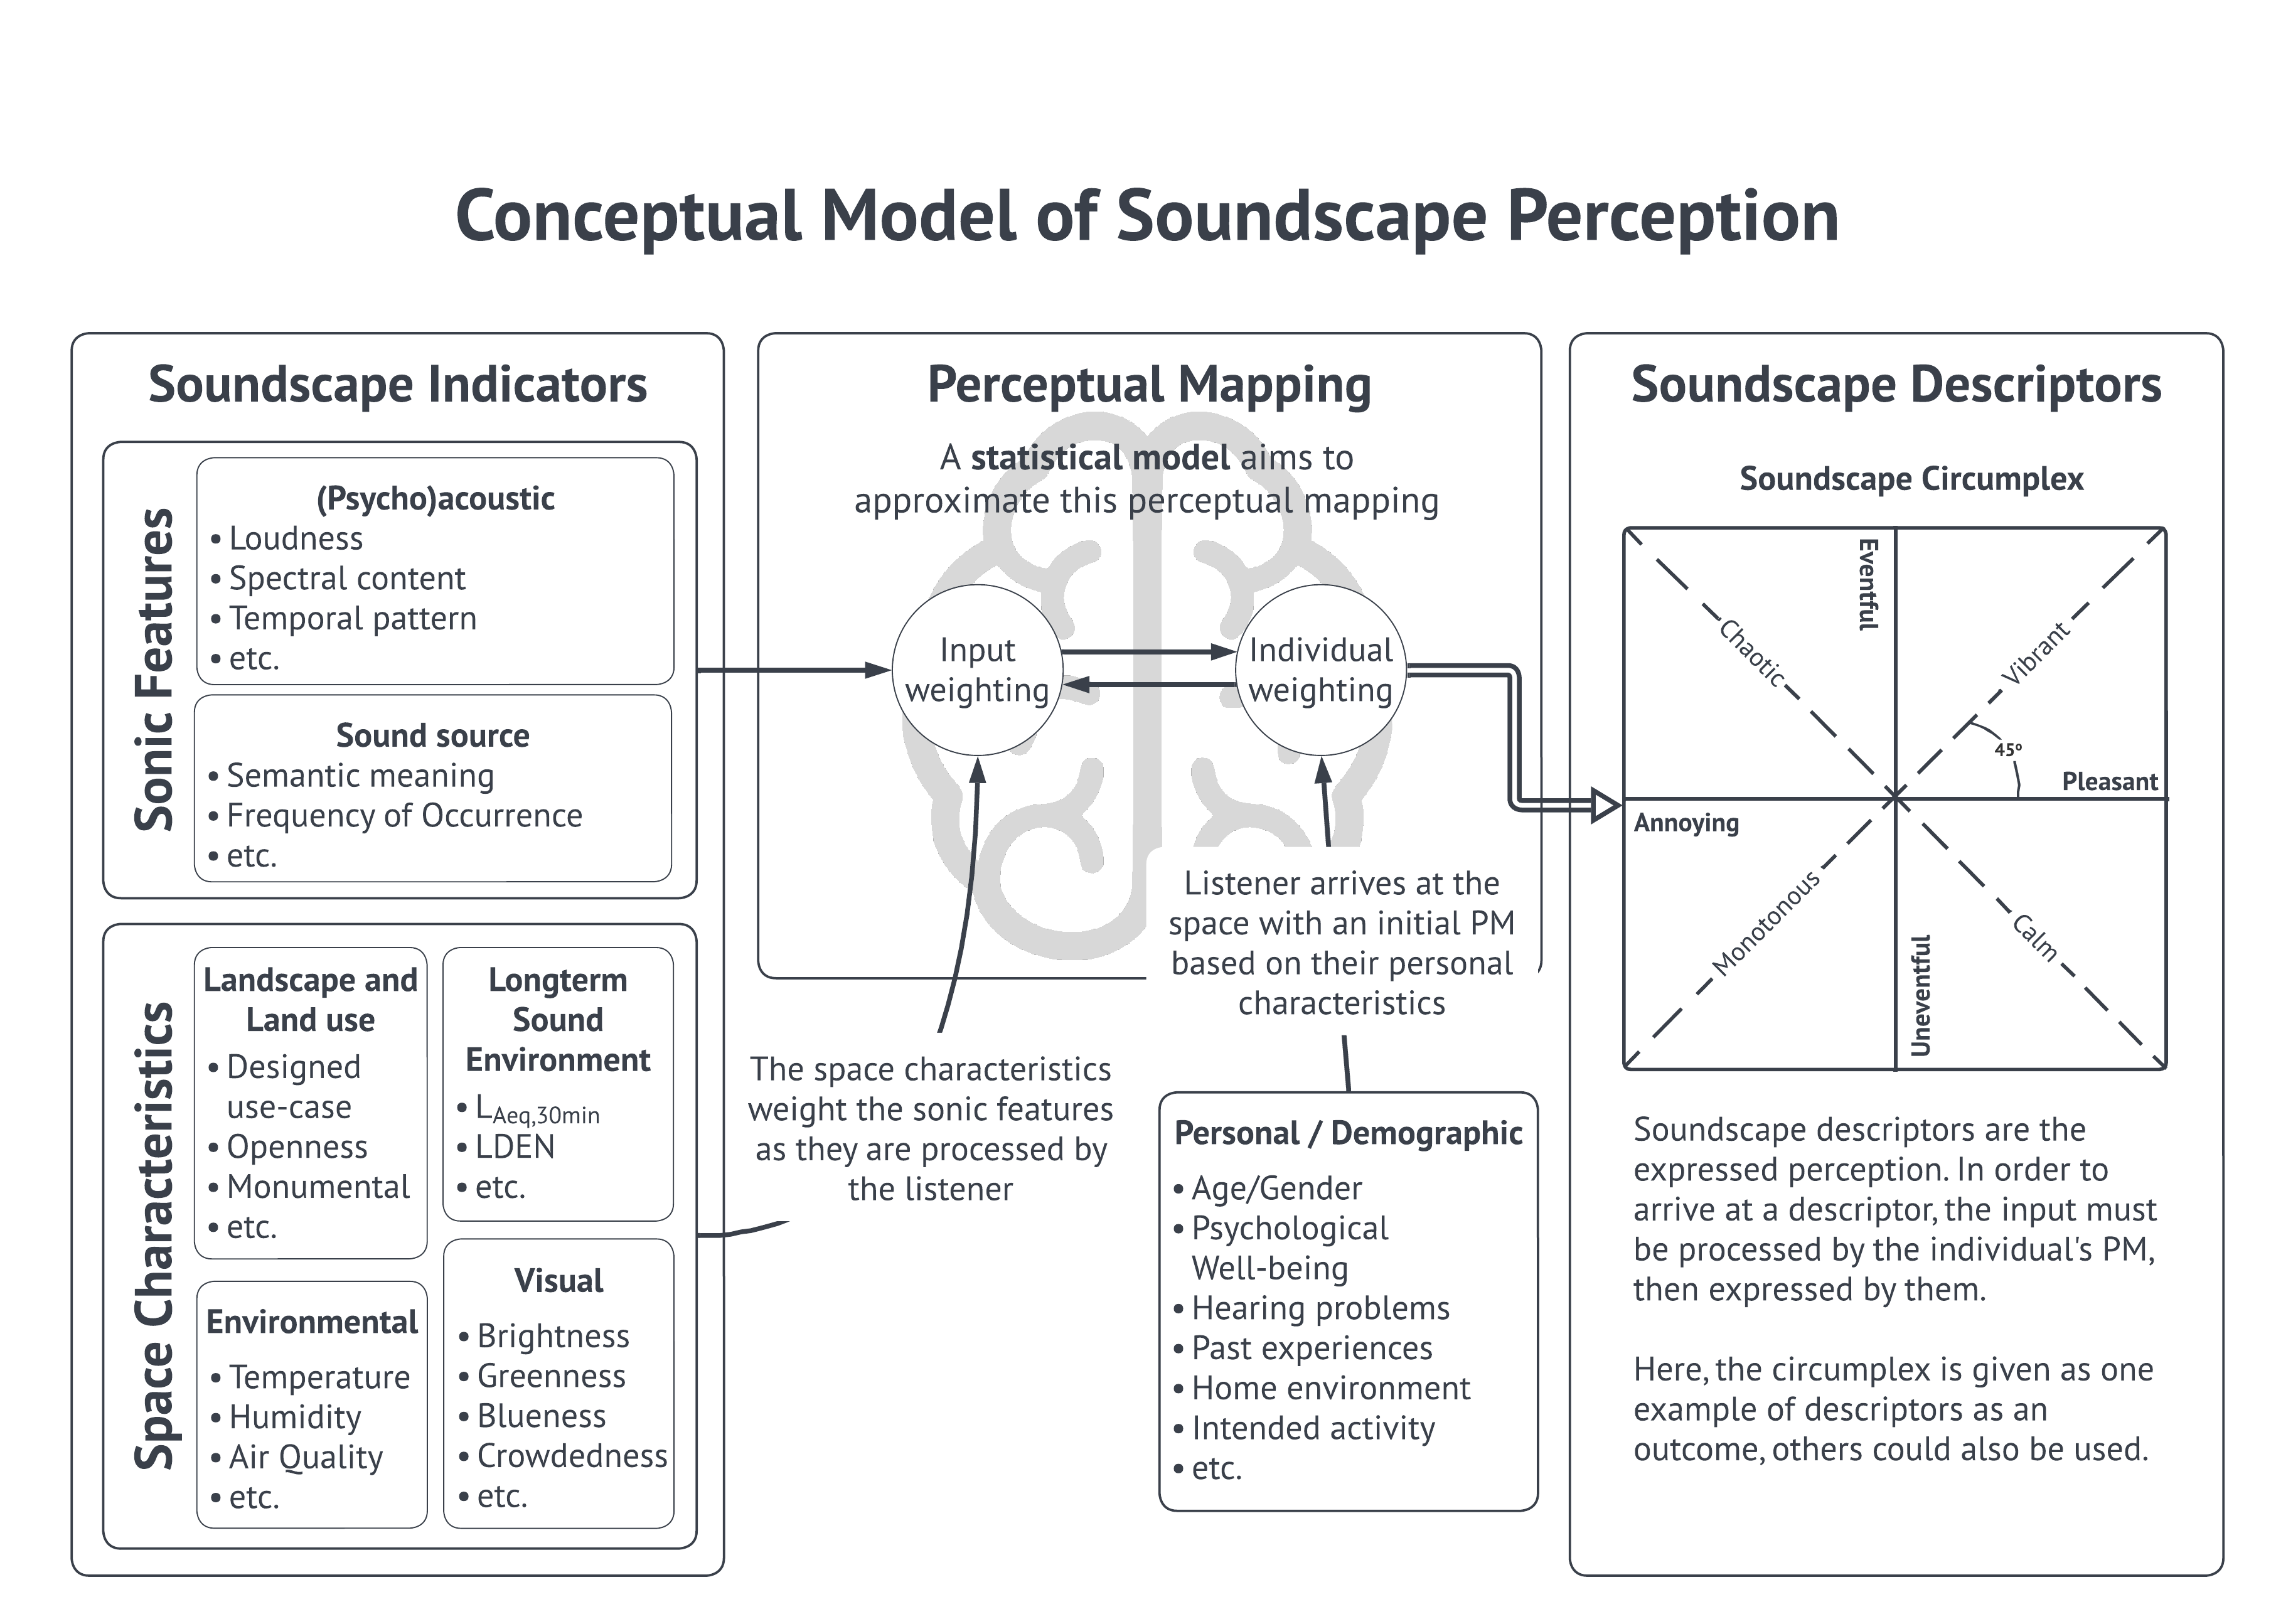
\includegraphics{Overall_Model_Concept_Diagram_2022-04-28.png}

}

\caption{\label{fig-model}The conceptual model of soundscape perception,
illustrating the perceptual mapping from physical inputs, through
personal experience, to soundscape descriptors. The role of the
statistical model is to attempt to approximate or reflect this
perceptual mappint. Reproduced with permission from
\citet{Mitchell2022Predictive}}

\end{figure}%

It should be made clear that this represents a very simplified view of
how a soundscape perception is formed, however it provides a useful
conceptual framework for the purposes of understanding and modelling how
someone's perception forms in response to their exposure to a space. One
way to consider the function of a statistical model of soundscape
perception is as replicating the perceptual mapping between soundscape
indicators and descriptors \citep{Lionello2021new}. As a person
experiences an urban space, they are exposed to an array of physical
inputs, these are then processed by the listener through their own
personal experience and mapped to their perception of that space. This
perception is then expressed through their description of this
experience of the soundscape. It is this mapping of physical inputs to
perceptual description which the statistical model aims to reflect. The
most successful model would then accurately replicate the general
perceptual mapping across the population.

\section{Applications in design and
mapping}\label{applications-in-design-and-mapping}

The soundscape approach faces several challenges in practical
applications which are unaddressed by current assessment methods, but
which may be solved through the development of a predictive modelling
framework. The first of these challenges is predicting how a change in
an existing sound environment will be reflected in the soundscape
perception. While it is possible in this scenario to measure the
existing soundscape perception via questionnaire surveys, if a change is
then introduced to the acoustic environment, it is so far impossible to
say what the resulting soundscape change would be. This question relates
strongly to the idea of soundscape interventions; where a particular
noise pollution challenge is addressed by introducing more pleasant
sounds (e.g.~a water feature), following the soundscape principle of
treating sound as a resource
\citep{Lavia2016Soundscape, Moshona2022What}. Predicting how much a
particular intervention would improve the soundscape (or, indeed whether
it would improve at all) is not yet possible with the retrospective
methods available.

Several studies have attempted to address this gap by developing machine
learning or statistical models of soundscape perception which are
focussed on prediction, rather than inference. An array of modelling
techniques are used, with linear regression being the most common
\citep{Lionello2020systematic}, and also including artificial neural
networks (ANN) \citep{PuyanaRomero2016Modelling, Yu2009Modeling} and
support vector regression (SVR)
\citep{Fan2016Automatic, Fan2017Emo, Giannakopoulos2019Athens}. However,
these studies have focussed primarily on using these models to
investigate the constructs of soundscape perception, with few efforts to
put the models themselves to use. \citet{Mitchell2021Investigating}
attempted to address this by both developing a predictive model and
applying it to an applied scenario where traditional assessment methods
were impractical. In a unique application, \citet{Ooi2022Probably}
created a predictive model of soundscape pleasantness which fed an
automated and reactive soundscape enhancement system
\citep{Watcharasupat2022Autonomous}.

Retrospective methods also struggle to capture the dynamics of the
soundscape in a space. Whether through the narrative interview method of
ISO/TS 12913-2 \citep{ISO12913Part2}, through soundwalks, or through in
situ questionnaires \citep{Mitchell2020Soundscape}, only the soundscape
during the particular period which the researchers are actively
investigating is captured. This makes it very difficult to determine
diurnal, seasonal, or yearly patterns of the soundscape. These patterns
may be driven by corresponding diurnal, seasonal, or yearly patterns in
the acoustic or visual environment, or by variations in how people
process and respond to the sound at different times of day/season/year.
Currently the only way to investigate any of these patterns is through
repeated surveys. Predictive modelling, on the other hand, could allow a
trained soundscape model to be paired with longterm monitoring methods
to track how a soundscape perception may change in response to changes
in the acoustic environment.

Similarly, a move towards modelling methods based on objective and/or
measurable factors would facilitate the application of mapping in
soundscape. While noise maps have become common in urban noise research
and legislation \citep{EEA2020Environmental, Gasco2020Social}, they can
be difficult to translate into a soundscape approach. The Environmental
Noise Directive (END) \citep{EuropeanUnion2002Directive}, first
implemented in 2002, is the main EU instrument to identify noise
pollution impacts and track urban noise levels across the EU. Its goals
were to determine the population's exposure to environmental noise, make
information on environmental noise available to the public, and prevent
and reduce environmental noise and its effects. In general, noise maps
are based on modelled traffic flows, from which decibel levels are
extrapolated and mapped, although interpolation and mobile measurement
methods have also been recently developed
\citep[see][]{Aumond2018Probabilistic}. Alternatively, they can be
produced using longterm SLMs or sensor networks. While these methods
have significant utility for tracking increases in urban noise levels
and are important for determining the health and societal impacts of
noise on a large scale, their restricted focus on noise levels alone
limits their scope and reduces the potential for identifying more
nuanced health and psychological effects of urban sound.

Several studies have attempted to bring soundscape to urban noise
mapping. The most notable of these attempts
\citep{Aumond2018Probabilistic, Aletta2015Soundscape, Hong2017Exploring, Kang2018Impact}
bring new, more sophisticated methods for mapping urban sound (not just
noise levels). For instance, all four present methods which map the
relative level of various sound sources, producing maps of the spatial
distribution of bird sounds, human voices, water sounds, etc. In
\citet{Aletta2015Soundscape} and \citet{Hong2017Exploring} the mapping
relied on soundscape surveys conducted in public spaces, then used
interpolation methods and basic relationships to the measured noise
levels to generate a map of the perceived soundscape over the entire
study space. \citet{Kang2018model}, after starting with survey
responses, attempted to create a prediction methods which relied only on
the audio recordings made in the space to create visual maps of the
predicted soundscape perception (i.e.~the perceptual attributes
'pleasant', 'calm', 'eventful', 'annoying', 'chaotic', 'monotonous').
According to the authors, the prediction and mapping model would follow
three steps: (1) sound sources recognition and profiling, (2) prediction
of the soundscape's perceptual attributes, and (3) implementation of
soundscape maps. Unfortunately, from the paper, it appears that the
prediction model results were not actually used for the mapping and,
again, the survey responses from 21 respondents were interpolated to
create the soundscape map. Their results indicated how a predictive
model could have been slotted into a mapping use-case, but this was
limited by (1) the relatively poor predictive performance for several of
the attributes, (2) the inability to automatically recognise sound
sources, and (3) a very limited dataset in terms of sample size and
variety of locations.

While the connection is not made to perception,
\citet{Aumond2018Probabilistic} focussed on creating sound maps which
can reflect the pattern of sound source emergences over time within a
city. By stochastically activating varying sound sources across their
map, they could map the percentage of time when a sound source emerges
from the overall complex sound environment. If a predictive soundscape
model which incorporates sound source information can be developed, then
the same procedure which led to their sound source emergence maps could
also feed the soundscape model, resulting in a map of predicted
perception over time.

Urban scale noise mapping and its implementation at the international
level has been crucial in highlighting the health impacts of urban noise
and in providing evidence for the negative cost of excess noise. Traffic
flow models of noise, large community noise surveys, and policy
requirements to track noise levels have all been necessary to reveal
these impacts. By creating predictive soundscape models, combined with
new tools and sensing capabilities from smart city efforts, we can bring
soundscape into these same realms. Without this, these large-scale
impact studies will be limited to valuing the negative cost of urban
noise, missing the potential value of positive soundscapes. By bringing
perception-based practice to the same scale and type of evidence, we can
expand urban sound research to consider a holistic view of urban spaces
and their impacts.

The broader use-case and need for such soundscape models and maps was
recently highlighted by \citet{Jiang2022Ten}, which opens the discussion
for how the value and impact of soundscapes should be measured and what
tools are needed to enable the valuation of policy interventions for
soundscapes. In response to Question 5, ``What soundscape metrics and
data will be needed?'', the authors make clear the necessity of
predictive soundscape models: ``Quantitative soundscape metrics that
link subjective perceptions to objective acoustic and contextual factors
will be needed, to enable monetisation while at the same time account
for the perception-based nature of soundscape.'' In addition, the
authors make a strong case for the need for soundscape indices:
``Despite the varied requirements for soundscape metrics and data
between and even within valuation methods, a standardised metric or set
of metrics, such as dB in noise valuation {[}. . . {]} will allow
comparison and integration of different studies and building compatible
evidence bases.''

\section{The Predictive Soundscape Model
Framework}\label{the-predictive-soundscape-model-framework}

Several forms and iterations of predictive models have been developed
\citep{Lionello2020systematic} and more recently they have been put to
use in real-world use cases
\citep{Mitchell2021Investigating, Watcharasupat2022Autonomous}. To
improve on these models and make them into a useful engineering tool, we
should establish a framework of overarching goals for models to achieve
and the resulting development constraints. In general, the goals we
define are related to how we might wish for models to be used and
deployed, while the constraints are practical limitations which may make
the performance of a given model less than ideal, but are necessary to
achieve the deployment goals.

\subsection{Goals}\label{goals}

Before defining what form a general practical predictive model should
take, we first need to make clear what the goals of such a model are, as
derived from the preceding discussion laying out why predictive models
are needed in soundscape.

\textbf{Accuracy} -- First, that it to a reasonable extent is successful
in predicting the collective perception \citep[see][]{Mitchell2022How}
of a soundscape. It should succeed at both indicating the central
tendency of the soundscape perception, but importantly it should also
inform the likely spread of perception among the population. The outcome
of the predictive model should not be focussed on predicting an
individual assessment; the goal is not the predict the perception of any
specific individual, but to reflect the public's perception of a public
space. In other words, ideally the model will result in an accurate
distribution of soundscape perceptions for the target population.

\textbf{Automation} -- Second, that it can be implemented automatically.
Once an initial setup is performed, such as identifying what location
the measurements are conducted in, the model should be capable of moving
from recorded information to predicted soundscape distribution without
human intervention. We need soundscape assessments to be able to be
performed instrumentally. This enables it to be applied to unmanned
uses, such as smart city sensors and soundscape mapping. It is
impractical to conduct soundscape surveys or soundwalks in every
location we wish to map and certainly not when we wish to see how these
locations change over longer periods of time. A predictive model should
allow us to survey these soundscapes remotely in order to extend
soundscape to city-scale assessments.

\textbf{Comparisons} -- Third, the model should enable us to test,
score, and compare proposed interventions. In a design context, it is
crucial that various strategies and interventions can be tested and that
the influencing factors can be identified. The model should assist the
user in highlighting what factor is limiting the success of a
soundscape, spark ideas for how to address it, and allow these ideas to
be tested. Several other useful features of predictive soundscape models
arise out of these goals and will be discussed later, but these form the
core goals of the framework.

\subsection{Constraints}\label{constraints}

If we accept that predictive models are necessary to advance a more
holistic approach to urban sound in smart cities, we must then define
the constraints of such a model. The goal here is to define a framework
for what is needed from a future model intended to be used in a smart
city sensors, soundscape mapping, or urban design context.

\textbf{Inputs} -- The first constraint is that the model must be based
on measurable factors. By this, we mean that the data which eventually
feeds into the predictive model should be collected via sensor
measurements of one sort or another; this could be acoustic sound level
measurements or recordings, environmental measurements, video
recordings, or GIS measurements, etc. What it certainly cannot include
is perceptual data. This is strictly a practical constraint -- for a
predictive model designed to be used in practice, there is no
justification to include other perceptual factors, such as perceived
greenness, derived from surveys but not whichever factor you desire to
predict. If the goal is to predict soundscape pleasantness and it is
necessary to survey people about the visual pleasantness, why not just
also survey them about the soundscape pleasantness directly? Certainly
this mix of perceptual data is useful in research and can elucidate the
relationship between the sonic and visual environments, but it is not
useful in a practical predictive context. Any results which arise from
research combining this sort of perceptual information must eventually
be translated into a component which can itself be measured or modelled.

\textbf{Calculation} -- The second constraint is that any analysis of
the measured data can be done automatically, without human intervention.
If the eventual goal is to deploy the model on continuously-running,
unmanned sensor nodes or to enable practical large-scale measurements,
the predictive model should be capable of operating with minimal human
input. This means, for instance that if the model includes information
about the sound source, this identification of the source should be
possible to do automatically (i.e.~through environmental sound
recognition).

A potential constraint for some applications is related to computation
time. Since one proposed application of a predictive soundscape model is
to embed the model on a WASN node, the model would then need to be able
to run on relatively low-power hardware such as a Raspberry Pi with a
reasonable latency. This would especially present an issue for those
models which rely on the combination of several psychoacoustic features
\citep[such as][]{Mitchell2021Investigating, Orga2021Multilevel}, since
these features are computationally intensive to calculate and several of
them may need to be computed for each time step of the model. Although
this is a real practical concern that should be addressed in the future,
for the sake of this initial definition of a general predictive model
used across many applications, we have not considered this a strict
constraint.

\textbf{Generalisability} -- The third constraint is for the model to be
generalisable to new locations. Ideally, it will be generalisable to new
and (to it) unfamiliar soundscape types, but the minimum requirement
should be that it can be applied to new locations which are otherwise
similar to those in the training data. This means that any factors which
are used to characterise the context provided by the location should be
distinguished from a simple label of the location and should instead be
derived from measurements of the location. In practice this could be
geographical or architectural characteristics of the space, a proposed
use-case of the space, or consistent visual characteristics of the space
such as the proportion of pavement to green elements. This is in
contrast to the model created in \citet{Mitchell2021Investigating} which
was constrained to be used only on those locations included in the
training data since it made use of a location label.

For this third point, some aspects of the first and second constraints
can be relaxed. Since this would only need to be defined once for a
location, definitions such as the use case of the space could be defined
by the person using the model. What is necessary is that the model and
its component location-context factors can be set up ahead of time by
the user, then the recording-level effects are able to be calculated
automatically. In a multi-level modelling (MLM) context (such as that
used in \citep{Mitchell2021Investigating}, this essentially amounts to
choosing the appropriate location-level coefficients ahead of time then
automatically calculating the features which are fed into those
coefficients (per constraint 1 \& 2).

\textbf{Robustness} -- Finally, the model should be robust to missing
components. If the original or full construction of the model depends on
demographic information of the population using the space, in cases
where this information is not available, it should be possible to omit
it and still obtain a reasonable result. Here we may define potential
`must-have' and `optional' factors. Given the amount of variance
explained by the various factors which have been considered in previous
predictive models, in-depth acoustic information is a must-have, while
demographic and personal factors are an optional factor where the
trade-off of losing 3\% of the explained variance in eventfulness
\citep{Erfanian2021Psychological} is accepted as reasonable. Based on
the results of \citet{Mitchell2021Investigating}, it would appear that
location-context is crucial for modelling the pleasantness, but not for
modelling the eventfulness. In order to determine the must-have factors
for characterising the location-context, more work will need to be done
to determine the appropriate input factors and their relative
importance.

\section{Making use of the predictions in
design}\label{making-use-of-the-predictions-in-design}

There are various potential methods for integrating the predictive
soundscape approach into a design and intervention setting. Not all
spaces can or should have the same soundscape and soundscapes should be
treated as dynamic, not static; identifying and creating an appropriate
soundscape for the particular use case of a space is crucial to guiding
its design. Proper forwardlooking design of a soundscape would involve
defining the desired collective perception in the space. In the
probabilistic soundscape approach from \citet{Mitchell2022How}, this can
be achieved by drawing the desired shape in the circumplex and testing
interventions which will bring the existing soundscape closer to the
desired perception. A soundscape may need to be perceived as vibrant
during the day and calm for some portion of the evening, meaning the
desired shape should primarily sit within the vibrant quadrant but have
some overlap into calm. This also enables designers to recognise the
limitations of their environment and acknowledge that it is not always
possible to transform a highly chaotic soundscape into a calm one. In
these cases, instead the focus should be placed on shifting the
perception to some degree in a positive direction.

\begin{figure}

\centering{

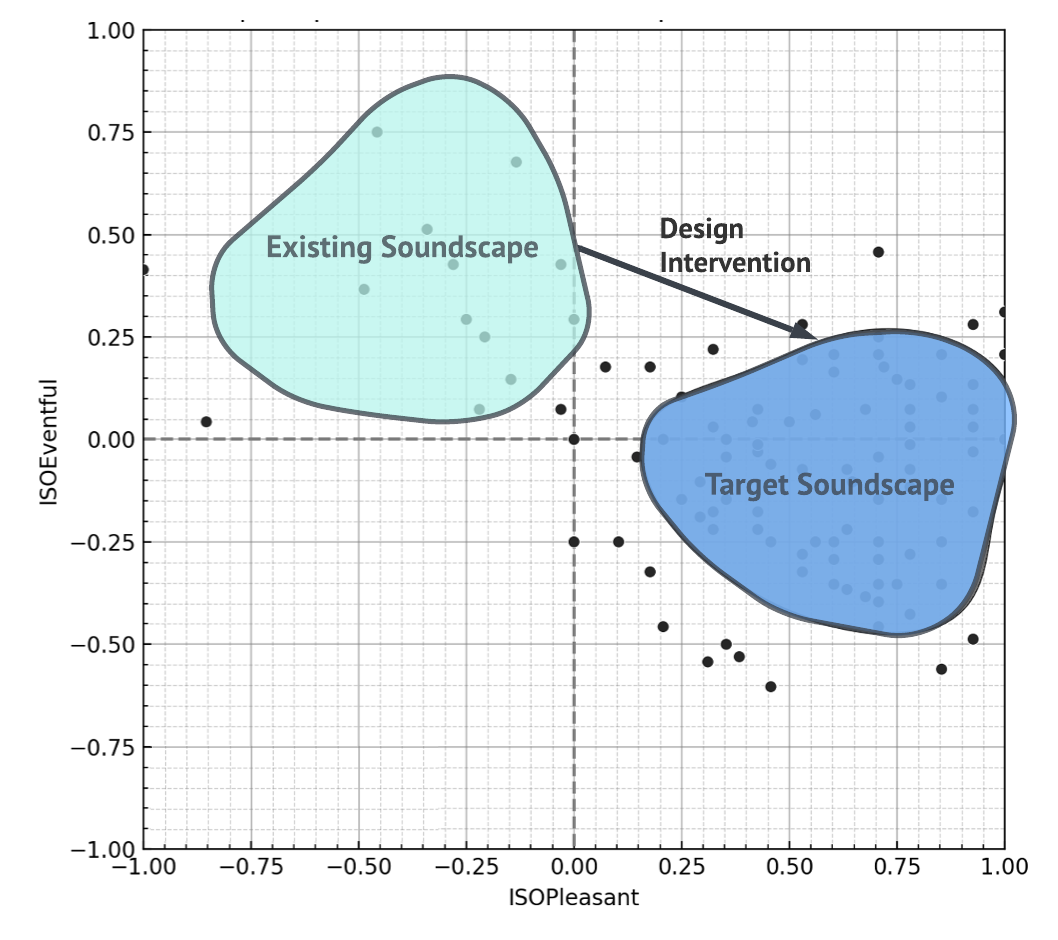
\includegraphics{CainCircumplexTarget.png}

}

\caption{\label{fig-cain}Adapted from \citet{Cain2013development}. Using
the soundscape circumplex shape for target-setting for soundscape
design. Reproduced with permission from \citet{Mitchell2022Predictive}.}

\end{figure}%

The most sophisticated method of setting design goals is therefore to
identify the desired shape which represents the variety of desired
outcomes, and focus on designs and interventions which are most
successful in matching the predicted outcome with that goal. This
strategy of defining the optimal soundscape as an area or a shape within
the 2-dimensional circumplex was previously illustrated by
\citet{Cain2013development}. In Figure~\ref{fig-cain}, we have adapted
Cain's Figure 6 to show how the shape of a target soundscape can be set
and the shape of the existing soundscape compared to it. The work of a
designer is then trialling intervention options which move the design
soundscape closer to the target soundscape.

\section{Towards Soundscape Indices}\label{towards-soundscape-indices}

Although the types of visualisations developed in
\citep{Mitchell2022How} and \citep{Cain2013development} are a powerful
tool for viewing, analysing, and discussing the multi-dimensional
aspects of soundscape perception, there are certainly cases where
simpler metrics are needed to aid discussion and to set design goals.
Within the practicalities of built environment projects, the
consequences and successes of a design often need to be quantifiable
within a single index. Whether to demonstrate performance indicators to
a client or to set and meet consistent policy requirements, numerical
ratings and/or rankings are necessary. This therefore necessitates the
creation of consistent and validated indices which indicate the degree
to which a proposal achieves a set design goal.

The challenge for creating a single number index lies in properly
combining the two-plus dimensions of soundscape perception with the
needs of a specific project into a single index. The obvious option
would be to ignore the multi-dimensionality and only score soundscape
designs on the basis of their pleasantness score (as done in
\citep{Ooi2022Probably}). However, this seems to ignore both the
significant importance of the eventfulness dimension in shaping the
character of a soundscape and the role of appropriateness in determining
the 'optimal soundscape' for a space. Ideally, a soundscape index (or
set of soundscape indices) would succeed at capturing all these aspects
into a single scoring metric.

\section{Conclusion}\label{conclusion}

The existing methods for soundscape assessment and measurement, such as
those given in the ISO 12913 series, have been focussed primarily on
determining the status quo of an environment. That is, they are able to
determine how the space is currently perceived, but offer little insight
into hypothetical environments. As such, they are less relevant for
design purposes, where a key goal is to determine how a space will be
perceived, not just how an existing space is perceived. The methods for
assessment outlined in \citet{ISO12913Part2} and for analysis given in
\citet{ISO12913Part3} are inherently limited to post hoc assessments of
an existing space. Since they are focussed on surveying people on their
experience of the environment, it stands that the space must already
exist for people to be able to experience. Toward this, and following
from the combination of perceptual and objective data collection
encouraged in \citet{ISO12913Part2}, the natural push from the design
perspective is towards 'predictive modelling'.


\renewcommand\refname{References}
  \bibliography{../../../FellowshipRefs.bib,../FellowshipRefs.bib}



\end{document}
